\section{Financial\_\-Monthly\_\-Sub\-Category  Class Reference}
\label{classFinancial__Monthly__SubCategory}\index{Financial_Monthly_SubCategory@{Financial\_\-Monthly\_\-Sub\-Category}}
{\tt \#include $<$dil2al.hh$>$}

Inheritance diagram for Financial\_\-Monthly\_\-Sub\-Category::\begin{figure}[H]
\begin{center}
\leavevmode
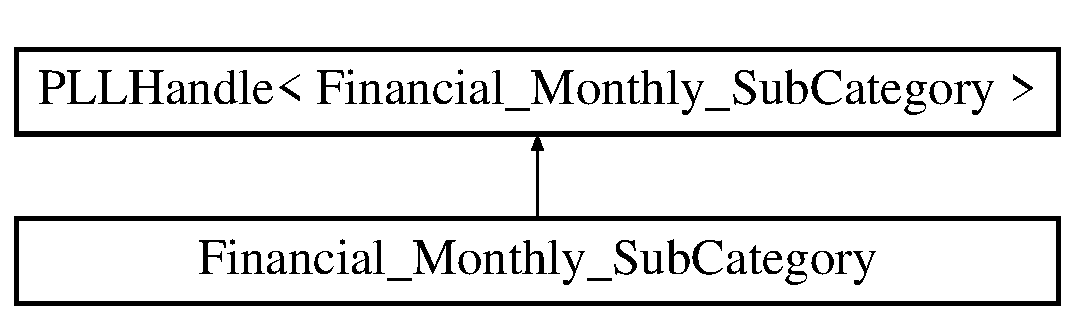
\includegraphics[height=2cm]{classFinancial__Monthly__SubCategory}
\end{center}
\end{figure}
\subsection*{Public Methods}
\begin{CompactItemize}
\item 
{\bf Financial\_\-Monthly\_\-Sub\-Category} ({\bf String} s, double r=0.0)
\item 
{\bf String} {\bf Sub\-Category} () const
\item 
Financial\_\-Monthly\_\-Sub\-Category $\ast$ {\bf Find\_\-Sub\-Category} ({\bf String} s) const
\item 
double {\bf Result} () const
\end{CompactItemize}
\subsection*{Protected Methods}
\begin{CompactItemize}
\item 
void {\bf add} (double e)
\end{CompactItemize}
\subsection*{Protected Attributes}
\begin{CompactItemize}
\item 
{\bf String} {\bf subcategory}
\item 
double {\bf result}
\end{CompactItemize}


\subsection{Constructor \& Destructor Documentation}
\index{Financial_Monthly_SubCategory@{Financial\_\-Monthly\_\-Sub\-Category}!Financial_Monthly_SubCategory@{Financial\_\-Monthly\_\-SubCategory}}
\index{Financial_Monthly_SubCategory@{Financial\_\-Monthly\_\-SubCategory}!Financial_Monthly_SubCategory@{Financial\_\-Monthly\_\-Sub\-Category}}
\subsubsection{\setlength{\rightskip}{0pt plus 5cm}Financial\_\-Monthly\_\-Sub\-Category::Financial\_\-Monthly\_\-Sub\-Category ({\bf String} {\em s}, double {\em r} = 0.0)\hspace{0.3cm}{\tt  [inline]}}\label{classFinancial__Monthly__SubCategory_a0}




Definition at line 1106 of file dil2al.hh.

References result.



\footnotesize\begin{verbatim}1106 : subcategory(s), result(r) {}
\end{verbatim}\normalsize 


\subsection{Member Function Documentation}
\index{Financial_Monthly_SubCategory@{Financial\_\-Monthly\_\-Sub\-Category}!add@{add}}
\index{add@{add}!Financial_Monthly_SubCategory@{Financial\_\-Monthly\_\-Sub\-Category}}
\subsubsection{\setlength{\rightskip}{0pt plus 5cm}void Financial\_\-Monthly\_\-Sub\-Category::add (double {\em e})\hspace{0.3cm}{\tt  [inline, protected]}}\label{classFinancial__Monthly__SubCategory_b0}




Definition at line 1104 of file dil2al.hh.

References result.

Referenced by Financial\_\-Monthly\_\-Category::add().



\footnotesize\begin{verbatim}1104 { result += e; }
\end{verbatim}\normalsize 
\index{Financial_Monthly_SubCategory@{Financial\_\-Monthly\_\-Sub\-Category}!Find_SubCategory@{Find\_\-SubCategory}}
\index{Find_SubCategory@{Find\_\-SubCategory}!Financial_Monthly_SubCategory@{Financial\_\-Monthly\_\-Sub\-Category}}
\subsubsection{\setlength{\rightskip}{0pt plus 5cm}Financial\_\-Monthly\_\-Sub\-Category $\ast$ Financial\_\-Monthly\_\-Sub\-Category::Find\_\-Sub\-Category ({\bf String} {\em s}) const}\label{classFinancial__Monthly__SubCategory_a2}




Definition at line 155 of file finances.cc.

References PLLHandle$<$ Financial\_\-Monthly\_\-Sub\-Category $>$::Next(), and subcategory.

Referenced by Financial\_\-Monthly\_\-Category::add().



\footnotesize\begin{verbatim}155                                                                                               {
156   if (subcategory==s) return const_cast<Financial_Monthly_SubCategory *>(this);
157   if (Next()) return Next()->Find_SubCategory(s);
158   return NULL;
159 }
\end{verbatim}\normalsize 
\index{Financial_Monthly_SubCategory@{Financial\_\-Monthly\_\-Sub\-Category}!Result@{Result}}
\index{Result@{Result}!Financial_Monthly_SubCategory@{Financial\_\-Monthly\_\-Sub\-Category}}
\subsubsection{\setlength{\rightskip}{0pt plus 5cm}double Financial\_\-Monthly\_\-Sub\-Category::Result () const\hspace{0.3cm}{\tt  [inline]}}\label{classFinancial__Monthly__SubCategory_a3}




Definition at line 1109 of file dil2al.hh.

References result.



\footnotesize\begin{verbatim}1109 { return result; }
\end{verbatim}\normalsize 
\index{Financial_Monthly_SubCategory@{Financial\_\-Monthly\_\-Sub\-Category}!SubCategory@{SubCategory}}
\index{SubCategory@{SubCategory}!Financial_Monthly_SubCategory@{Financial\_\-Monthly\_\-Sub\-Category}}
\subsubsection{\setlength{\rightskip}{0pt plus 5cm}{\bf String} Financial\_\-Monthly\_\-Sub\-Category::Sub\-Category () const\hspace{0.3cm}{\tt  [inline]}}\label{classFinancial__Monthly__SubCategory_a1}




Definition at line 1107 of file dil2al.hh.



\footnotesize\begin{verbatim}1107 { return subcategory; }
\end{verbatim}\normalsize 


\subsection{Member Data Documentation}
\index{Financial_Monthly_SubCategory@{Financial\_\-Monthly\_\-Sub\-Category}!result@{result}}
\index{result@{result}!Financial_Monthly_SubCategory@{Financial\_\-Monthly\_\-Sub\-Category}}
\subsubsection{\setlength{\rightskip}{0pt plus 5cm}double Financial\_\-Monthly\_\-Sub\-Category::result\hspace{0.3cm}{\tt  [protected]}}\label{classFinancial__Monthly__SubCategory_n1}




Definition at line 1103 of file dil2al.hh.

Referenced by add(), Financial\_\-Monthly\_\-Sub\-Category(), and Result().\index{Financial_Monthly_SubCategory@{Financial\_\-Monthly\_\-Sub\-Category}!subcategory@{subcategory}}
\index{subcategory@{subcategory}!Financial_Monthly_SubCategory@{Financial\_\-Monthly\_\-Sub\-Category}}
\subsubsection{\setlength{\rightskip}{0pt plus 5cm}{\bf String} Financial\_\-Monthly\_\-Sub\-Category::subcategory\hspace{0.3cm}{\tt  [protected]}}\label{classFinancial__Monthly__SubCategory_n0}




Definition at line 1102 of file dil2al.hh.

Referenced by Find\_\-Sub\-Category().

The documentation for this class was generated from the following files:\begin{CompactItemize}
\item 
{\bf dil2al.hh}\item 
{\bf finances.cc}\end{CompactItemize}
